\newcommand{\titulus}{\nomenFesti{In Nativitate S. Ioannis Baptistæ.}
\celebratio{Duplex 1. classis.}}
\newcommand{\festum}{Ioannes Baptista}
\newcommand{\aequus}{Ioannes Baptista}
\newcommand{\festumveldominica}{Ioannes Baptista}
\newcommand{\solemnis}{Ioannes Baptista}
\newcommand{\lectioi}{\pars{Lectio I.}

\noindent Sermo sancti Augustíni Epíscopi in natáli Iohánnis Baptístæ.

\noindent Natálem sancti Iohánnis, fratres caríssimi, hódie celebrámus, quod nulli unquam sanctórum légimus fuísse concéssum. Solíus enim Dómini et beáti Iohánnis dies nativitátis in univérso mundo celebrátur et cólitur. Illum enim stérilis péperit; istum virgo concépit. In Elísabeth sterílitas víncitur, in beáta María conceptiónis consuetúdo mutátur. Elísabeth virum cognoscéndo fílium génuit; María ángelo crédidit, et concépit. Hóminem concépit Elísabeth, et hóminem María; sed Elísabeth solum hóminem, María Deum et hóminem.}
\newcommand{\lectioii}{\pars{Lectio II.}

\noindent Quid sibi vult ergo Iohánnes? Unde interpósitus, unde præmíssus? Magnus ígitur Iohánnes, cuius magnitúdini étiam salvátor testimónium pérhibet, dicens: Non surréxit inter natos mulíerum maior Iohánne Baptísta. Præcéllit cunctis, éminet univérsis; antecéllit prophétas, supergréditur patriárchas; et quisquis de mulíere natus est, inférior est Iohánne. Dicit fortásse áliquis: Si inter natos mulíerum Iohánnes maior est, maior est salvatóre. Absit. Iohánnes enim natus mulíeris, Christus autem vírginis natus est; ille corruptíbilis úteri sínibus effúsus est, iste impollútæ vulvæ flore progénitus.}
\newcommand{\lectioiii}{\pars{Lectio III.}

\noindent Ideo autem cum Iohánnis nativitáte Dómini generátio deputátur, ne Dóminus extra veritátem videátur conditiónis humánæ: si comparétur homínibus Iohánnes, præmíssus est ante Deum. Tanta in illo excelléntia erat, tanta grátia, ut ipse putátus sit Christus. Quid ergo dixit de Christo? Nos omnes de plenitúdine eius accépimus. Quid est: nos omnes? Ergo prophétæ, patriárchæ, apóstoli, quotquot sancti, et ante incarnatiónem præmíssi, vel ab incarnáto missi, omnes nos de plenitúdine eius accépimus: nos vasa sumus, ille fons est. Si ergo intelléximus mystérium, fratres mei, Iohánnes homo est, Christus Deus est: humiliétur homo, et exaltétur Deus, secúndum illud, quod de Dómino ipse Iohánnes dixit: Illum opórtet créscere, me autem mínui. Ut humiliarétur homo, eo ei die natus est Iohánnes, quo incípiunt decréscere dies: ut exaltétur Deus, eo die natus est Christus, quo incípiunt créscere dies.}
\newcommand{\lectioiv}{\pars{Lectio IV.}

\noindent Magnum sacraméntum, fratres caríssimi. Ideo celebrámus natálem Iohánnis, sicut et Christi, quia et ipsa natívitas plena est mystério. Quo mystério, nisi humilitátis nostræ; sicut natívitas Christi plena est mystério altitúdinis nostræ? Ergo in hómine minuámur, ut in Deo crescámus; in nobis humiliémur, ut in illo exaltémur; humiliétur humána præsúmptio, ut crescat divína miserátio. Nam huius rei sacraméntum étiam in passiónibus ambórum implétum est. Ut minuétur homo, caput Iohánnis abscínditur; ut exaltétur Deus, Christus in ligno suspénditur. Quare autem beátum Iohánnem Dóminus et salvátor noster lucérnam esse díxerit, et quare eum mitti ante se volúerit, bréviter, si iubétis, caritátis vestræ áuribus intimábo.}
\newcommand{\lectiov}{\pars{Lectio V.}

\noindent Perfécta Christi grátia semper confirmétur in nobis. Præmíssus est enim velut vox ante verbum, lucérna ante solem, præco ante iúdicem, servus ante dóminum, amícus ante sponsum. Et quia univérsum mundum peccatórum ténebræ et nox infidelitátis opprésserat, et solem iustítiæ aspícere non valébat, beátus Iohánnes quasi lucérna præmíttitur, ut cordis óculi, qui lippitúdine iniquitátis oppréssi magnum et verum lumen vidére non póterant, ad lumen lucérnæ primum quasi ténuem splendórem vidére consuéscerent; et paulátim peccatórum núbilo remóto, et infidelitátis humóre digésto, adveniénte Christo, ab illo cælésti lúmine lætificáre possent pótius quam torquéri. Sicut enim lippiéntes óculos ad vidéndum próvocas, si exíguum splendórem lucérnæ osténderis; et ámplius crúcias, si lumen magnum ingésseris: ita Dóminus et Salvátor noster, qui est lumen verum, nisi prius beátum Iohánnem velut lucérnam prætermítteret, claritátem illíus totus mundus sustinére non posset.}
\newcommand{\lectiovi}{\pars{Lectio VI.}

\noindent Loquátur Iohánnes et dicat: ego vox clamántis in desérto. Vox erat, quia Verbi Dei Spíritu replebátur. Sicut sermo vocis quodam modo ministério ac vehículo ad audiéntem a loquénte transmíttitur, ita ille Christum sonans, Verbi erat miníster et pórtitor. Sanctus, inquam, Iohánnes typum in se legis, quæ Christum longe per signa et iudícia monstrábat, osténdit; et ídeo misit ad Christum duos de discípulis suis. Isti duo discípuli a Iohánne ad Christum missi, forte duo pópuli sunt, quorum unus ex Iudǽis crédidit, alter ex géntibus. Iohánnes dírigit ad Christum, lex mittit ad grátiam, et per evangélii fidem, véterem desíderat ástrui veritátem. Nos vero, fratres charíssimi, ut tam sanctam festivitátem non solum corporáli, sed étiam spirituáli cum gáudio celebráre possímus, secúndum vires nostros ad dandas eleemósynas, et ad tenéndam cum ómnibus pacem nostros ánimos præparémus: et ab omni scurrilitáte vel turpilóquio non solum nosmetipsos, sed et omnem famíliam nostram et univérsos ad nos pertinéntes pro amóre Dei et zelo sanctæ disciplínæ prohibére totis víribus laborémus, nec permittámus voluptuósos quosque solemnitátem sanctam cántica luxuriósa proferéndo pollúere.  Tunc enim pro nobis sanctus Iohánnes quidquid petiérimus póterit obtinére, si nos festivitátem suam pacíficos, sóbrios, castos, absque ullo turpilóquio cognóverit celebráre. Hæc ergo,  fratres charíssimi, pro patérna sollicitúdo súggero: nam Deo propítio ita de vestra devotióne confído, quod non solum vos ipsos, sed étiam omnes qui ad vos pértinent, cum omne honestáte castos sobriósque conservétis. Unde Deo grátias agens súpplico, ut qui vobis dedit ea, quæ sancta sunt fidéliter incípere, concédat vobis felícem perseverántiam custodíre, qui cum Patre et Spíritu Sancto vivit et regnat, Deus, in sǽcula sæculórum. Amen.}
\newcommand{\lectiovii}{\pars{Lectio VII.} \scriptura{Io. 6, 56-59}

\noindent Léctio sancti Evangélii secúndum Lucam..

\noindent In illo témpore: Elísabeth implétum est tempus pariéndi, et péperit fílium. Et audiérunt vicíni et cognáti eius, quod magnificávit Dóminus misericórdiam suam cum illa, et congratulabántur ei. Et réliqua.

\vspace{4mm}

\noindent Ex homilía venerábilis Bedæ presbýteri in nativitáte sancti Iohánnis Baptístæ.

\noindent Præcursóris Dómini natívitas, sicut sacratíssima lectiónis evangélicæ prodit história, multa miraculórum sublimitáte refúlget, quia nimírum decébat, ut ille, quo maior inter natos mulíerum nemo surréxit maióre præ céteris sanctis in ipso mox ortu virtútum iúbare clarésceret. Senes ac diu infecúndi paréntes dono nobilíssimæ prolis exsúltant. Ipsi patri, quem incredúlitas mutum reddíderat, ad salutándum novæ præcónem grátiæ os et lingua reserátur. Nec solum facúltas Deum benedicéndi restitúitur, sed de eo étiam prophetándi virtus augétur. Excitáti vero fama facti omnes vicíni admiratióne ac metu percellúntur ómnium, qui audiére circumquáque ad advéntum novi prophétæ corda percellúntur.}
\newcommand{\lectioviii}{\pars{Lectio VIII.}

\noindent Unde mérito sancta per orbem ecclésia, quæ tot beatórum mártyrum victórias, quibus ingréssum regni cæléstis meruére frequéntat, huius tantúmmodo post Dómini étiam nativitátis diem celebráre consuévit. Quod nullátenus sine evangélica auctoritáte in consuetúdinem venísse credéndum est, sed atténtius ánimo recordendum, quia sicut nato Dómino pastóribus appárens ángelus ait: Ecce evangelízo vobis gáudium magnum, quod erit omni pópulo, quia natus est nobis hódie salvátor, qui est Christus Dóminus, ita étiam ángelus nascitúrum Zacharíæ prǽdicans Iohánnem. Et erit tibi gáudium, inquit, et exsultátio, et multi in nativitáte eius gaudébunt. Et erit magnus coram Dómino. Iure ígitur utriúsque natívitas festa devotióne celebrátur, sed in illíus tamquam in Christi Dómini, tamquam in salvatóris mundi, tamquam in Fílii Dei omnipoténtis, tamquam in solis iustítiæ nativitáte omni pópulo gáudium evangelizátur, in huius autem tamquam in præcursóris Dómini, in servi Dómini exímii, in lucérnæ ardéntis et lucéntis exórtu multi gavísi esse memorántur.}
\newcommand{\lectioix}{\pars{Lectio IX.}

\noindent Iste magnus coram Dómino esse narrátur, de illo prophéta testátur, quóniam magnus Dóminus et laudábilis nimis, et magnitúdinis eius non est finis, Iste peccatórum consórtia declínans, ab omni quod inebriáre potest, abstinébat, ille inter peccatóres conversátus, peccáti omnis immúnis permánsit. Hic adhuc ex útero matris Spíritu Sancto replétus est, in illo hábitat omnis plenitúdo divinitátis corporáliter, qui dono sui Spíritus sedem sibi úteri virginális, in quo carnem suscíperet, ipse consecrávit. Iste multos filiórum Isráhel ad Dóminum suo témpore prædicándo convértit. Ille multos cotídie de univérsis per orbem natiónibus ad suam fidem et caritátem intérius illustrándo convértere non desístit. Hic in Spíritu et virtúte Helíæ præcéssit ante illum, ut plebem eius aqua baptízans ad suscipiéndum eum, ubi apparéret, docéret esse perféctam. Huic succéssit ille in Spíritu et virtúte Dei Patris, ut plebem suam Spíritu sancto et igne baptízans ad vidéndam fáciem patris sui donáret esse perféctam.}
% LuaLaTeX

\documentclass[a4paper, twoside, 12pt]{article}
\usepackage[latin]{babel}
%\usepackage[landscape, left=3cm, right=1.5cm, top=2cm, bottom=1cm]{geometry} % okraje stranky
%\usepackage[landscape, a4paper, mag=1166, truedimen, left=2cm, right=1.5cm, top=1.6cm, bottom=0.95cm]{geometry} % okraje stranky
\usepackage[landscape, a4paper, mag=1400, truedimen, left=0.5cm, right=0.5cm, top=0.5cm, bottom=0.5cm]{geometry} % okraje stranky

\usepackage{fontspec}
\setmainfont[FeatureFile={junicode.fea}, Ligatures={Common, TeX}, RawFeature=+fixi]{Junicode}
%\setmainfont{Junicode}

% shortcut for Junicode without ligatures (for the Czech texts)
\newfontfamily\nlfont[FeatureFile={junicode.fea}, Ligatures={Common, TeX}, RawFeature=+fixi]{Junicode}

\usepackage{multicol}
\usepackage{color}
\usepackage{lettrine}
\usepackage{fancyhdr}

% usual packages loading:
\usepackage{luatextra}
\usepackage{graphicx} % support the \includegraphics command and options
\usepackage{gregoriotex} % for gregorio score inclusion
\usepackage{gregoriosyms}
\usepackage{wrapfig} % figures wrapped by the text
\usepackage{parcolumns}
\usepackage[contents={},opacity=1,scale=1,color=black]{background}
\usepackage{tikzpagenodes}
\usepackage{calc}
\usepackage{longtable}
\usetikzlibrary{calc}

\setlength{\headheight}{14.5pt}

% Commands used to produce a typical "Conventus" booklet

\newenvironment{titulusOfficii}{\begin{center}}{\end{center}}
\newcommand{\dies}[1]{#1

}
\newcommand{\nomenFesti}[1]{\textbf{\Large #1}

}
\newcommand{\celebratio}[1]{#1

}

\newcommand{\hora}[1]{%
\vspace{0.5cm}{\large \textbf{#1}}

\fancyhead[LE]{\thepage\ / #1}
\fancyhead[RO]{#1 / \thepage}
\addcontentsline{toc}{subsection}{#1}
}

% larger unit than a hora
\newcommand{\divisio}[1]{%
\begin{center}
{\Large \textsc{#1}}
\end{center}
\fancyhead[CO,CE]{#1}
\addcontentsline{toc}{section}{#1}
}

% a part of a hora, larger than pars
\newcommand{\subhora}[1]{
\begin{center}
{\large \textit{#1}}
\end{center}
%\fancyhead[CO,CE]{#1}
\addcontentsline{toc}{subsubsection}{#1}
}

% rubricated inline text
\newcommand{\rubricatum}[1]{\textit{#1}}

% standalone rubric
\newcommand{\rubrica}[1]{\vspace{3mm}\rubricatum{#1}}

\newcommand{\notitia}[1]{\textcolor{red}{#1}}

\newcommand{\scriptura}[1]{\hfill \small\textit{#1}}

\newcommand{\translatioCantus}[1]{\vspace{1mm}%
{\noindent\footnotesize \nlfont{#1}}}

% pruznejsi varianta nasledujiciho - umoznuje nastavit sirku sloupce
% s prekladem
\newcommand{\psalmusEtTranslatioB}[3]{
  \vspace{0.5cm}
  \begin{parcolumns}[colwidths={2=#3}, nofirstindent=true]{2}
    \colchunk{
      \input{#1}
    }

    \colchunk{
      \vspace{-0.5cm}
      {\footnotesize \nlfont
        \input{#2}
      }
    }
  \end{parcolumns}
}

\newcommand{\psalmusEtTranslatio}[2]{
  \psalmusEtTranslatioB{#1}{#2}{8.5cm}
}


\newcommand{\canticumMagnificatEtTranslatio}[1]{
  \psalmusEtTranslatioB{#1}{temporalia/extra-adventum-vespers/magnificat-boh.tex}{12cm}
}
\newcommand{\canticumBenedictusEtTranslatio}[1]{
  \psalmusEtTranslatioB{#1}{temporalia/extra-adventum-laudes/benedictus-boh.tex}{10.5cm}
}

% volne misto nad antifonami, kam si zpevaci dokresli neumy
\newcommand{\hicSuntNeumae}{\vspace{0.5cm}}

% prepinani mista mezi notovymi osnovami: pro neumovane a neneumovane zpevy
\newcommand{\cantusCumNeumis}{
  \setgrefactor{17}
  \global\advance\grespaceabovelines by 5mm%
}
\newcommand{\cantusSineNeumas}{
  \setgrefactor{17}
  \global\advance\grespaceabovelines by -5mm%
}

% znaky k umisteni nad inicialu zpevu
\newcommand{\superInitialam}[1]{\gresetfirstlineaboveinitial{\small {\textbf{#1}}}{\small {\textbf{#1}}}}

% pars officii, i.e. "oratio", ...
\newcommand{\pars}[1]{\textbf{#1}}

\newenvironment{psalmus}{
  \setlength{\parindent}{0pt}
  \setlength{\parskip}{5pt}
}{
  \setlength{\parindent}{10pt}
  \setlength{\parskip}{10pt}
}

%%%% Prejmenovat na latinske:
\newcommand{\nadpisZalmu}[1]{
  \hspace{2cm}\textbf{#1}\vspace{2mm}%
  \nopagebreak%

}

% mode, score, translation
\newcommand{\antiphona}[3]{%
\hicSuntNeumae
\superInitialam{#1}
\includescore{#2}

#3
}
 % Often used macros
%%%% Preklady jednotlivych zpevu (nektere se opakuji, a je dobre mit je
% vsechny na jedne hromade)

\newcommand{\trOratioAnteOfficium}{\translatioCantus{Otevři, Pane, má ústa, abych chválil tvé svaté jméno.
Očisti mé srdce od všech marnivých, zvrácených a~jiných myšlenek, osvěť rozum, rozněť cit,
abych mohl důstojně, soustředěně a~zbožně recitovat a~vysloužil si být
vyslyšen před tváří tvé velebnosti. Skrze Krista…}}

\newcommand{\trOratioPostOfficium}{\translatioCantus{\textit{Následující modlitbu
opatřil pro ty, kdo ji zbožně vyřknou po hodinkách, zesnulý papež Lev X.
odpustky za hříchy vzniklé při konání hodinek z~lidské křehkosti. Říká se
vkleče.}
Svatosvaté a~nerozdílné Trojici, ukřižovanému lidství našeho Pána Ježíše
Krista, přeblažené a~přeslavné plodné neporušenosti vždy Panny Marie
i~souhrnu všech svatých buď ode všeho stvoření věčná chvála, čest a~sláva, nám
pak buď dáno odpuštění všech hříchů, po nekonečné věky věků. Amen.}}

% HOURS ---

\newcommand{\trAntI}{\translatioCantus{Jasné narození slavné Panny Marie,
z pokolení (dosl. ze semene) Abrahámova, vzešlé z kmene Judova, z rodu Davidova.}}
\newcommand{\trAntII}{\translatioCantus{Dnes je Narození svaté Panny 
Marie, jejíž předrahý život osvěcuje všechny církve.}}

\newcommand{\trAntIII}{\translatioCantus{Maria, jež vzešla 
z královského rodu, září; myslí i duchem ji zbožně prosíme, aby 
nám pomáhala svými přímluvami.}}

\newcommand{\trAntIV}{\translatioCantus{Srdcem i duchem pějme Kristu 
k slávě o této svaté slavnosti vznešené Rodičky Boží Marie.}}

\newcommand{\trAntV}{\translatioCantus{Příjemně \notitia{?} 
oslavujme Narození blahoslavené Marie,
aby se ona za nás přimlouvala u Pána Ježíše Krista.}}

\newcommand{\trCapituli}{\translatioCantus{Před věky, na počátku mě stvořil, potrvám věčně. Ve svatém Stanu jsem před ním konala službu.}}

\newcommand{\trRespVesp}{\translatioCantus{Buď zdráva, Maria,
plná milosti: \grestar{} Pán s tebou. \Vbardot{} Požehnaná jsi mezi ženami,
a požehnaný plod života (ve smyslu lůna, břicha) tvého.}}

\newcommand{\trVersus}{\translatioCantus{\Vbardot{} Dnes je Narození svaté Panny Marie. \Rbardot{} Jejíž předrahý život osvěcuje všechny církve.}}

\newcommand{\trAntMagnificatI}{\translatioCantus{Konejme památku
veledůstojného narození slavné Panny Marie,
jíž se dostalo mateřské důstojnosti bez ztráty panenské cudnosti.}}

% Tento preklad je vice nez nejisty a ani alternativy, ktere jsem
% videl, me nepresvedcily...
\newcommand{\trAntBenedictus}{\translatioCantus{Slavnostně slavme 
dnešní narození Marie, vždy Panny a Rodičky Boží: v něm se objevuje
vysokost trůnu (totiž Marie, trůnu Božího Syna), aleluja.}}

\newcommand{\trAntMagnificatII}{\translatioCantus{Tvé narození,
Bohorodičko Panno, vyhlásilo radost celému světu:
z tebe totiž vzešlo Slunce spravedlnosti, Kristus, náš Bůh:
jenž zrušil kletbu a dal nám požehnání: přemohl smrt a dal nám život věčný.}}

\newcommand{\trOrationis}{\translatioCantus{Prosíme tě, Bože, 
uděl svým služebníkům dar nebeské milosti,
aby těm, jimž slehnutím blahoslavené Panny vyvstal počátek spásy, 
slavnost k poctě jejího narození přinesla
rozhojnění pokoje.
Skrze tvého Syna, našeho Pána Ježíše Krista, který s tebou žije a kraluje,
Bůh, v jednotě Ducha svatého po všechny věky věků.}}

\newcommand{\trFideliumAnimae}{\translatioCantus{\Vbardot{} Duše věrných ať pro
milosrdenství Boží odpočívají v~pokoji. \Rbardot{} Amen.}}

% Completorium

\newcommand{\trJubeDomne}{\translatioCantus{Rač, pane, požehnat.}}

\newcommand{\trComplBenedictio}{\translatioCantus{Pokojnou noc a~svatou smrt
nechť nám dopřeje všemohoucí Pán. \Rbardot{} Amen.}}

\newcommand{\trComplLectioBr}{\translatioCantus{Buďte střízliví, bděte.
Váš protivník Ďábel obchází jako lev řvoucí a~hledá, koho by pohltil.
Postavte se proti němu pevní ve víře.  Ale ty, Pane, smiluj se nad námi.
\Rbardot{} Bohu díky.}}

\newcommand{\trComplAntI}{\translatioCantus{Rač se smilovati nade mnou,
Hospodine, a vyslyš mou modlitbu.}}

\newcommand{\trComplCapituli}{\translatioCantus{Jsi přece, Hospodine,
uprostřed nás a~jmenujeme se po tobě.  Neopouštěj nás, Pane, náš Bože.}}

\newcommand{\trRespCompl}{\translatioCantus{Do tvých rukou, Pane, \grestar{}
poroučím svého ducha. \Vbardot{} Ty mne zachráníš, Pane, Bože věrný.}}

\newcommand{\trComplVersus}{\translatioCantus{\Vbardot{} Střez mne jako zřítelnici oka,
aleluja. \Rbardot{} Ve stínu svých křídel uschovej mne, aleluja.}}

\newcommand{\trAntSalvaNos}{\translatioCantus{Ochraňuj nás, Pane, když
bdíme, a~buď s~námi, když spíme, ať bdíme s~Kristem a~odpočíváme v~pokoji.}}

\newcommand{\trComplOrationis}{\translatioCantus{Zavítej, prosíme, Pane, sem
do našeho příbytku a~daleko od něj zažeň všechny úklady nepřítele. Ať tu
bydlí tví svatí andělé a~tvoje požehnání buď nad ním stále. Skrze…}}

\newcommand{\trSalveRegina}{\translatioCantus{Zdrávas Královno, matko
milosrdenství, živote, sladkosti a naděje naše, buď zdráva!
K tobě voláme, vyhnaní synové Evy,
k tobě vzdycháme, lkajíce a plačíce
v tomto slzavém údolí.
A proto, orodovnice naše,
obrať k nám své milosrdné oči
a Ježíše, požehnaný plod života svého,
nám po tomto putování ukaž,
ó milostivá, ó přívětivá,
ó přesladká, Panno Maria!}}

\newcommand{\trOraProNobis}{\translatioCantus{\Vbardot{} 
Oroduj za nás, svatá Boží Rodičko,
\Rbardot{} aby nám Kristus dal účast na svých zaslíbeních.}}

% Matutinum

\newcommand{\trMatInvitatorium}{\translatioCantus{}}

\newcommand{\trMatVeniteA}{\translatioCantus{Pojďte, chvalme s~radostí Pána,
s~jásotem slavme Boha, svou spásu; předstupme před tvář jeho s~díky, písně plesu pějme jemu.}}

\newcommand{\trMatVeniteB}{\translatioCantus{Neboť Bůh veliký jest Hospodin, a~král nade všecky bohy.
Jsouť v~jeho ruce všecky hlubiny země, temena hor jsou majetek jeho.}}

\newcommand{\trMatVeniteC}{\translatioCantus{Jehoť jest moře, neb on je učinil; i~souš
je dílo jeho rukou. Pojďme, klanějme se, padněme, klekněme před Pánem, svým
tvůrcem. Jeť on Pán, náš Bůh, a~my jsme lid, jejž on vodí a~ovce, jež pase.}}

\newcommand{\trMatVeniteD}{\translatioCantus{Kéž byste poslechli dnes hlasu jeho:
,,Nezatvrzujte svých srdcí jak v~Hádce, jak v~Pokušení na poušti, kde vaši otcové pokoušeli mne,
zkoušeli mne, ač vídali skutky mé.``}}

\newcommand{\trMatVeniteE}{\translatioCantus{Čtyřicet roků mrzel jsem se na to pokolení
a~řekl jsem: ,,Lid je to myslí stále bloudící``! Oni však nechtěli znáti mé cesty, takže jsem
přisáhl ve svém hněvu: ,,Nedojdou odpočinku mého!\mbox{}``}}

\newcommand{\trMatAntI}{\translatioCantus{}}

\newcommand{\trMatAntII}{\translatioCantus{}}

\newcommand{\trMatAntIII}{\translatioCantus{}}

\newcommand{\trMatVersusI}{\translatioCantus{}}

\newcommand{\trMatAbsolutioI}{\translatioCantus{Vyslyš Pane Ježíši Kriste
prosby svých služebníků \gredagger{} a~smiluj se nad námi, \grestar{} jenž
s~Otcem a~Duchem…}}

\newcommand{\trMatBenedictioI}{\translatioCantus{Rač, pane, požehnat.
Věčný Otec nám stále žehnej. \Rbardot{} Amen.}}

\newcommand{\trMatLecI}{\translatioCantus{Kéž by mě zulíbal polibky svých úst. 
Tvé milování je nad víno lahodnější;
vybraně voní tvé voňavky;
rozlévající se olej je tvé jméno,
proto tě dívky milují.
Strhni mě za sebou, poběžme!
Král mě uvedl do svých komnat;
budeš nám radostí a jásotem.
Víc než víno oslavíme tvé milování;
věru po právu jsi milován!
Snědá jsem, a přece krásná, jeruzalémské dcery,
jako stany kedarské,
jako šalmské závěsy.
}}

\newcommand{\trMatRespI}{\translatioCantus{}}

\newcommand{\trMatBenedictioII}{\translatioCantus{Rač, pane, požehnat.
Jednorozený Boží Syn nám žehnej \grestar{} a nám pomáhej. \Rbardot{} Amen.}}

\newcommand{\trMatLecII}{\translatioCantus{Nehleďte na mou osmahlou pleť:
to mě slunce ožehlo.
Synové mé matky se na mne rozzlobili,
poslali mě hlídat vinice.
A svou vinici, tu jsem nehlídala!
Pověz mi tedy, ty, jehož miluje mé srdce:
kam zavedeš své stádo pást,
kde ho necháš za poledne odpočívat?
Abych už nebloudila jako tulačka
poblíž stád druhů tvých.
Nevíš-li to, nejrásnější z žen,
jdi po stopách stáda
a kůzlata svá zaveď, ať se pasou
poblíž obydlí pastýřů.
Ke své klisně zapřažené do vozu faraonova
tebe, mé milá, přirovnávám.
Stále krásné jsou tvé líce s náušnicemi
i tvé hrdlo v náhrdelnících.}}

\newcommand{\trMatRespII}{\translatioCantus{}}

\newcommand{\trMatBenedictioIII}{\translatioCantus{Rač, pane, požehnat.
Milost Ducha Svatého ať osvítí nám smysly \grestar{} i srdce. \Rbardot{} Amen.}}

\newcommand{\trMatLecIII}{\translatioCantus{Zhotovíme ti zlaté náušnice
a kuličky ze stříbra.
Když král stoluje,
vydechuje můj nard svou vůni.
Můj milý je polštářek s myrhou,
jenž mi odpočívá mezi ňadry.
Můj milý je hrozen šáchoru
ve vinicích v Engadi.
Jak jsi krásná, milá moje,
jak jsi krásná!
Tvé oči jsou holubice.
Jak jsi krásný, můj milý,
jak líbezný!
Naše lože je samá zeleň.
Trámoví našeho domu je z cedru,
naše ostění z cypřiše.}}

\newcommand{\trMatRespIII}{\translatioCantus{}}

\newcommand{\trMatAntIV}{\translatioCantus{}}

\newcommand{\trMatAntV}{\translatioCantus{}}

\newcommand{\trMatAntVI}{\translatioCantus{}}

\newcommand{\trMatVersusII}{\translatioCantus{}}

\newcommand{\trMatAbsolutioII}{\translatioCantus{
Tvá milost a laskavost nechť nám pomáhá, jenž žiješ a vládneš s Otcem a Svatým Duchem na věky věků.}}

\newcommand{\trMatBenedictioIV}{\translatioCantus{Rač, pane, požehnat.
Bůh Otec všemohoucí, \grestar{} buď k nám milostivý a odpouštějící. \Rbardot{} Amen.}}

\newcommand{\trMatLecIV}{\translatioCantus{}}

\newcommand{\trMatRespIV}{\translatioCantus{}}

\newcommand{\trMatBenedictioV}{\translatioCantus{}}

\newcommand{\trMatLecV}{\translatioCantus{}}

\newcommand{\trMatRespV}{\translatioCantus{}}

\newcommand{\trMatBenedictioVI}{\translatioCantus{Rač, pane, požehnat.
Bůh rozněť v nás oheň své lásky. \Rbardot{} Amen.}}

\newcommand{\trMatLecVI}{\translatioCantus{}}

\newcommand{\trMatRespVI}{\translatioCantus{}}

\newcommand{\trMatAntVII}{\translatioCantus{}}

\newcommand{\trMatAntVIII}{\translatioCantus{}}

\newcommand{\trMatAntIX}{\translatioCantus{}}

\newcommand{\trMatVersusIII}{\translatioCantus{}}

\newcommand{\trMatAbsolutioIII}{\translatioCantus{Z okovů našich hříchů,
\grestar{} vysvoboď nás všemohoucí a milosrdný Pán. \Rbardot{} Amen.}}

\newcommand{\trMatBenedictioVII}{\translatioCantus{Rač, pane, požehnat.
Čtení evangelia nechť je nám \grestar{} spásou a ochranou. \Rbardot{} Amen.}}

\newcommand{\trMatLecVIIa}{\translatioCantus{
  Rodokmen Ježíše Krista, syna Davidova, syna Abrahámova:
  Abrahám zplodil Izáka,
  Izák zplodil Jakuba.}}

\newcommand{\trMatLecVIIb}{\translatioCantus{}}

\newcommand{\trMatRespVII}{\translatioCantus{}}

\newcommand{\trMatBenedictioVIII}{\translatioCantus{Rač, pane, požehnat.
\Rbardot{} Amen.}}

\newcommand{\trMatLecVIII}{\translatioCantus{}}

\newcommand{\trMatRespVIII}{\translatioCantus{}}

\newcommand{\trMatBenedictioIX}{\translatioCantus{Rač, pane, požehnat.
Do společnosti občanů nebes \grestar{} ať nás dovede král andělů.
\Rbardot{} Amen.}}

\newcommand{\trMatLecIX}{\translatioCantus{}}

% from the Czech Liturgia horarum
\newcommand{\trTeDeum}{\begin{translatioMulticol}{3}

Bože, tebe chválíme, 
tebe, Pane, velebíme.

Tebe, věčný Otče, 
oslavuje celá země.

Všichni andělé, 
cherubové i~serafové,

všechny mocné nebeské zástupy 
bez ustání volají:

Svatý, Svatý, Svatý, 
Pán, Bůh zástupů.

Plná jsou nebesa i~země 
tvé vznešené slávy.

Oslavuje tě 
sbor tvých apoštolů,

chválí tě 
velký počet proroků,

vydává o~tobě svědectví 
zástup mučedníků;

a~po celém světě 
vyznává tě tvá církev:

neskonale velebný, 
všemohoucí Otče,

úctyhodný Synu Boží, 
pravý a~jediný,

božský Utěšiteli, 
Duchu svatý.

Kriste, Králi slávy, 
tys od věků Syn Boha Otce;

abys člověka vykoupil, 
stal ses člověkem a~narodil ses z~Panny;

zlomil jsi osten smrti 
a~otevřel věřícím nebe;

sedíš po Otcově pravici 
a~máš účast na jeho slávě.

Věříme, že přijdeš soudit, 

a~proto tě prosíme:
přispěj na pomoc svým služebníkům, 
vždyť jsi je vykoupil svou předrahou krví;

dej, ať se radují s~tvými svatými 
ve věčné slávě.

Zachraň, Pane, svůj lid, žehnej svému dědictví, 
veď ho a~stále pozvedej.

Každý den tě budeme velebit 
a~chválit tvé jméno po všechny věky.

Pomáhej nám i~dnes, 
ať se nedostaneme do područí hříchu.

Smiluj se nad námi, Pane, 
smiluj se nad námi.

Ať spočine na nás tvé milosrdenství, 
jak doufáme v~tebe.

Pane, k~tobě se utíkáme, 
ať nejsme zahanbeni na věky. 
\end{translatioMulticol}}

\newcommand{\trMatEvangelium}{\translatioCantus{
  Rodokmen Ježíše Krista, syna Davidova, syna Abrahámova:
  Abrahám zplodil Izáka,
  Izák zplodil Jakuba,
  Jakub zplodil Judu a jeho bratry,
  Juda zplodil Farese a Zaru z Tamary,
  Fares zplodil Esroma,
  Esrom zplodil Arama,
  Aram zplodil Aminadaba,
  Aminadab zplodil Naasona,
  Naason zplodil Salmona,
  Salmon zplodil Boaze z Rahaby,
  Boaz zplodil Jobeda z Rut,
  Jobed zplodil Jessea,
  Jesse zplodil krále Davida.
  David zplodil Šalomouna z Uriášovy ženy,
  Šalomoun zplodil Roboama,
  Roboam zplodil Abiu,
  Abia zplodil Asu,
  Asa zplodil Josafata,
  Josafat zplodil Jorama,
  Joram zplodil Oziáše,
  Oziáš zplodil Joatama,
  Joatam zplodil Achaze,
  Achaz zplodil Ezechiáše,
  Ezechiáš zplodil Manasesa,
  Manases zplodil Amona,
  Amon zplodil Josiáše,
  Josiáš zplodil Jechoniáše a jeho bratry;
  tehdy došlo k odvlečení do Babylonu.
  Po odvlečení do Babylonu:
  Jechoniáš zplodil Salatiela,
  Salatiel zplodil Zorobabela,
  Zorobabel zplodil Abiuda,
  Abiud zplodil Eljakima,
  Eljakim zplodil Azora,
  Ator zplodil Sadoka,
  Sadok zplodil Achima,
  Achim zplodil Eliuda,
  Eliud zplodil Eleazara,
  Eleatar zplodil Matana,
  Matan zplodil Jakuba,
  Jakub zplodil Josefa, manžela Marie,
  z níž se narodil Ježíš, který se nazývá Kristus.}}

\newcommand{\trTeDecetLaus}{\translatioCantus{Tobě chvála, Tobě zpěvy, Tobě
sláva, Bohu Otci i~Synu i~Svatému Duchu, na věky věků. \Rbardot{} Amen.}}

% MASS ---

\newcommand{\trIntroitus}{\translatioCantus{Radujme se všichni
v Pánu, slavíce svátek ke cti Panny Marie: z něj se radují andělé
a spoluchválí Božího Syna. \textit{\color{red}Žl.} Má ústa vydala dobré slovo,
přednáším svá díla králi.}}

\newcommand{\trGraduale}{\translatioCantus{Požehnaná a ctihodná jsi,
Panno Maria: nedotčená (co do panenství) jsi byla shledána matkou
Spasitele. \Vbardot{} Panno Boží Rodičko, ten, jehož nepojme ani celý svět,
se uzavřel do tvých útrob, když se stal člověkem.}}

\newcommand{\trAlleluia}{\translatioCantus{Aleluja. \Vbardot{} Skvělá slavnost
slavné Panny Marie, z pokolení (dosl. ze semene) Abrahámova, vzešlé z kmene 
Judova, z rodu Davidova.}}

\newcommand{\trOffertorium}{\translatioCantus{Blažená jsi, Panno Maria,
tys nosila Stvořitele všeho; porodila jsi toho, který tě utvořil,
a na věky zůstáváš Pannou.}}

\newcommand{\trCommunio}{\translatioCantus{Budou mě blahoslavit
všechna pokolení, protože mi učinil veliké věci ten, který je mocný.}}

% LITTLE HOURS ---

\newcommand{\trVersusTertia}{\translatioCantus{\Vbardot{} \Rbardot{}}}

\newcommand{\trCapituliEtSic}{\translatioCantus{
Tak jsem se usadila na Sionu a v milovaném městě jsem nalezla odpočinek,
v Jeruzalémě vykonávám svou moc.
Zakořenila jsem u lidu plného slývy, na panství Páně, v jeho dědictví.}}

\newcommand{\trVersusSexta}{\translatioCantus{\Vbardot{} \Rbardot{}}}

\newcommand{\trCapituliInPlateis}{\translatioCantus{
Na planině jako skořicovník a akant jsem vydávala vůni, jako vybraná myrha
jsem voněla.}}

\newcommand{\trVersusNona}{\translatioCantus{\Vbardot{} \Rbardot{}}}
 % Czech translations of the proper texts

\newcommand{\annusEditionis}{2020}

%%%% Vicekrat opakovane kousky

\newcommand{\anteOrationem}{
  \rubrica{Ante Orationem, cantatur a Superiore:}

  \pars{Supplicatio Litaniæ.}

  \cuminitiali{}{temporalia/supplicatiolitaniae.gtex}

  \pars{Oratio Dominica.}

  \cuminitiali{}{temporalia/oratiodominica.gtex}

  \rubrica{Deinde dicitur ab Hebdomadario:}

  \cuminitiali{}{temporalia/dominusvobiscum-solemnis.gtex}

  \rubrica{In choro monialium loco Dominus vobiscum dicitur:}

  \sineinitiali{temporalia/domineexaudi.gtex}
}

\setlength{\columnsep}{30pt} % prostor mezi sloupci

%%%%%%%%%%%%%%%%%%%%%%%%%%%%%%%%%%%%%%%%%%%%%%%%%%%%%%%%%%%%%%%%%%%%%%%%%%%%%%%%%%%%%%%%%%%%%%%%%%%%%%%%%%%%%
\begin{document}

% Here we set the space around the initial.
% Please report to http://home.gna.org/gregorio/gregoriotex/details for more details and options
\grechangedim{afterinitialshift}{2.2mm}{scalable}
\grechangedim{beforeinitialshift}{2.2mm}{scalable}
\grechangedim{interwordspacetext}{0.22 cm plus 0.15 cm minus 0.05 cm}{scalable}%
\grechangedim{annotationraise}{-0.2cm}{scalable}

% Here we set the initial font. Change 38 if you want a bigger initial.
% Emit the initials in red.
\grechangestyle{initial}{\color{red}\fontsize{38}{38}\selectfont}

\pagestyle{empty}

%%%% Titulni stranka
\begin{titulusOfficii}
\titulus
\end{titulusOfficii}

% graphic
%\vspace{1.5cm}
%\begin{center}
%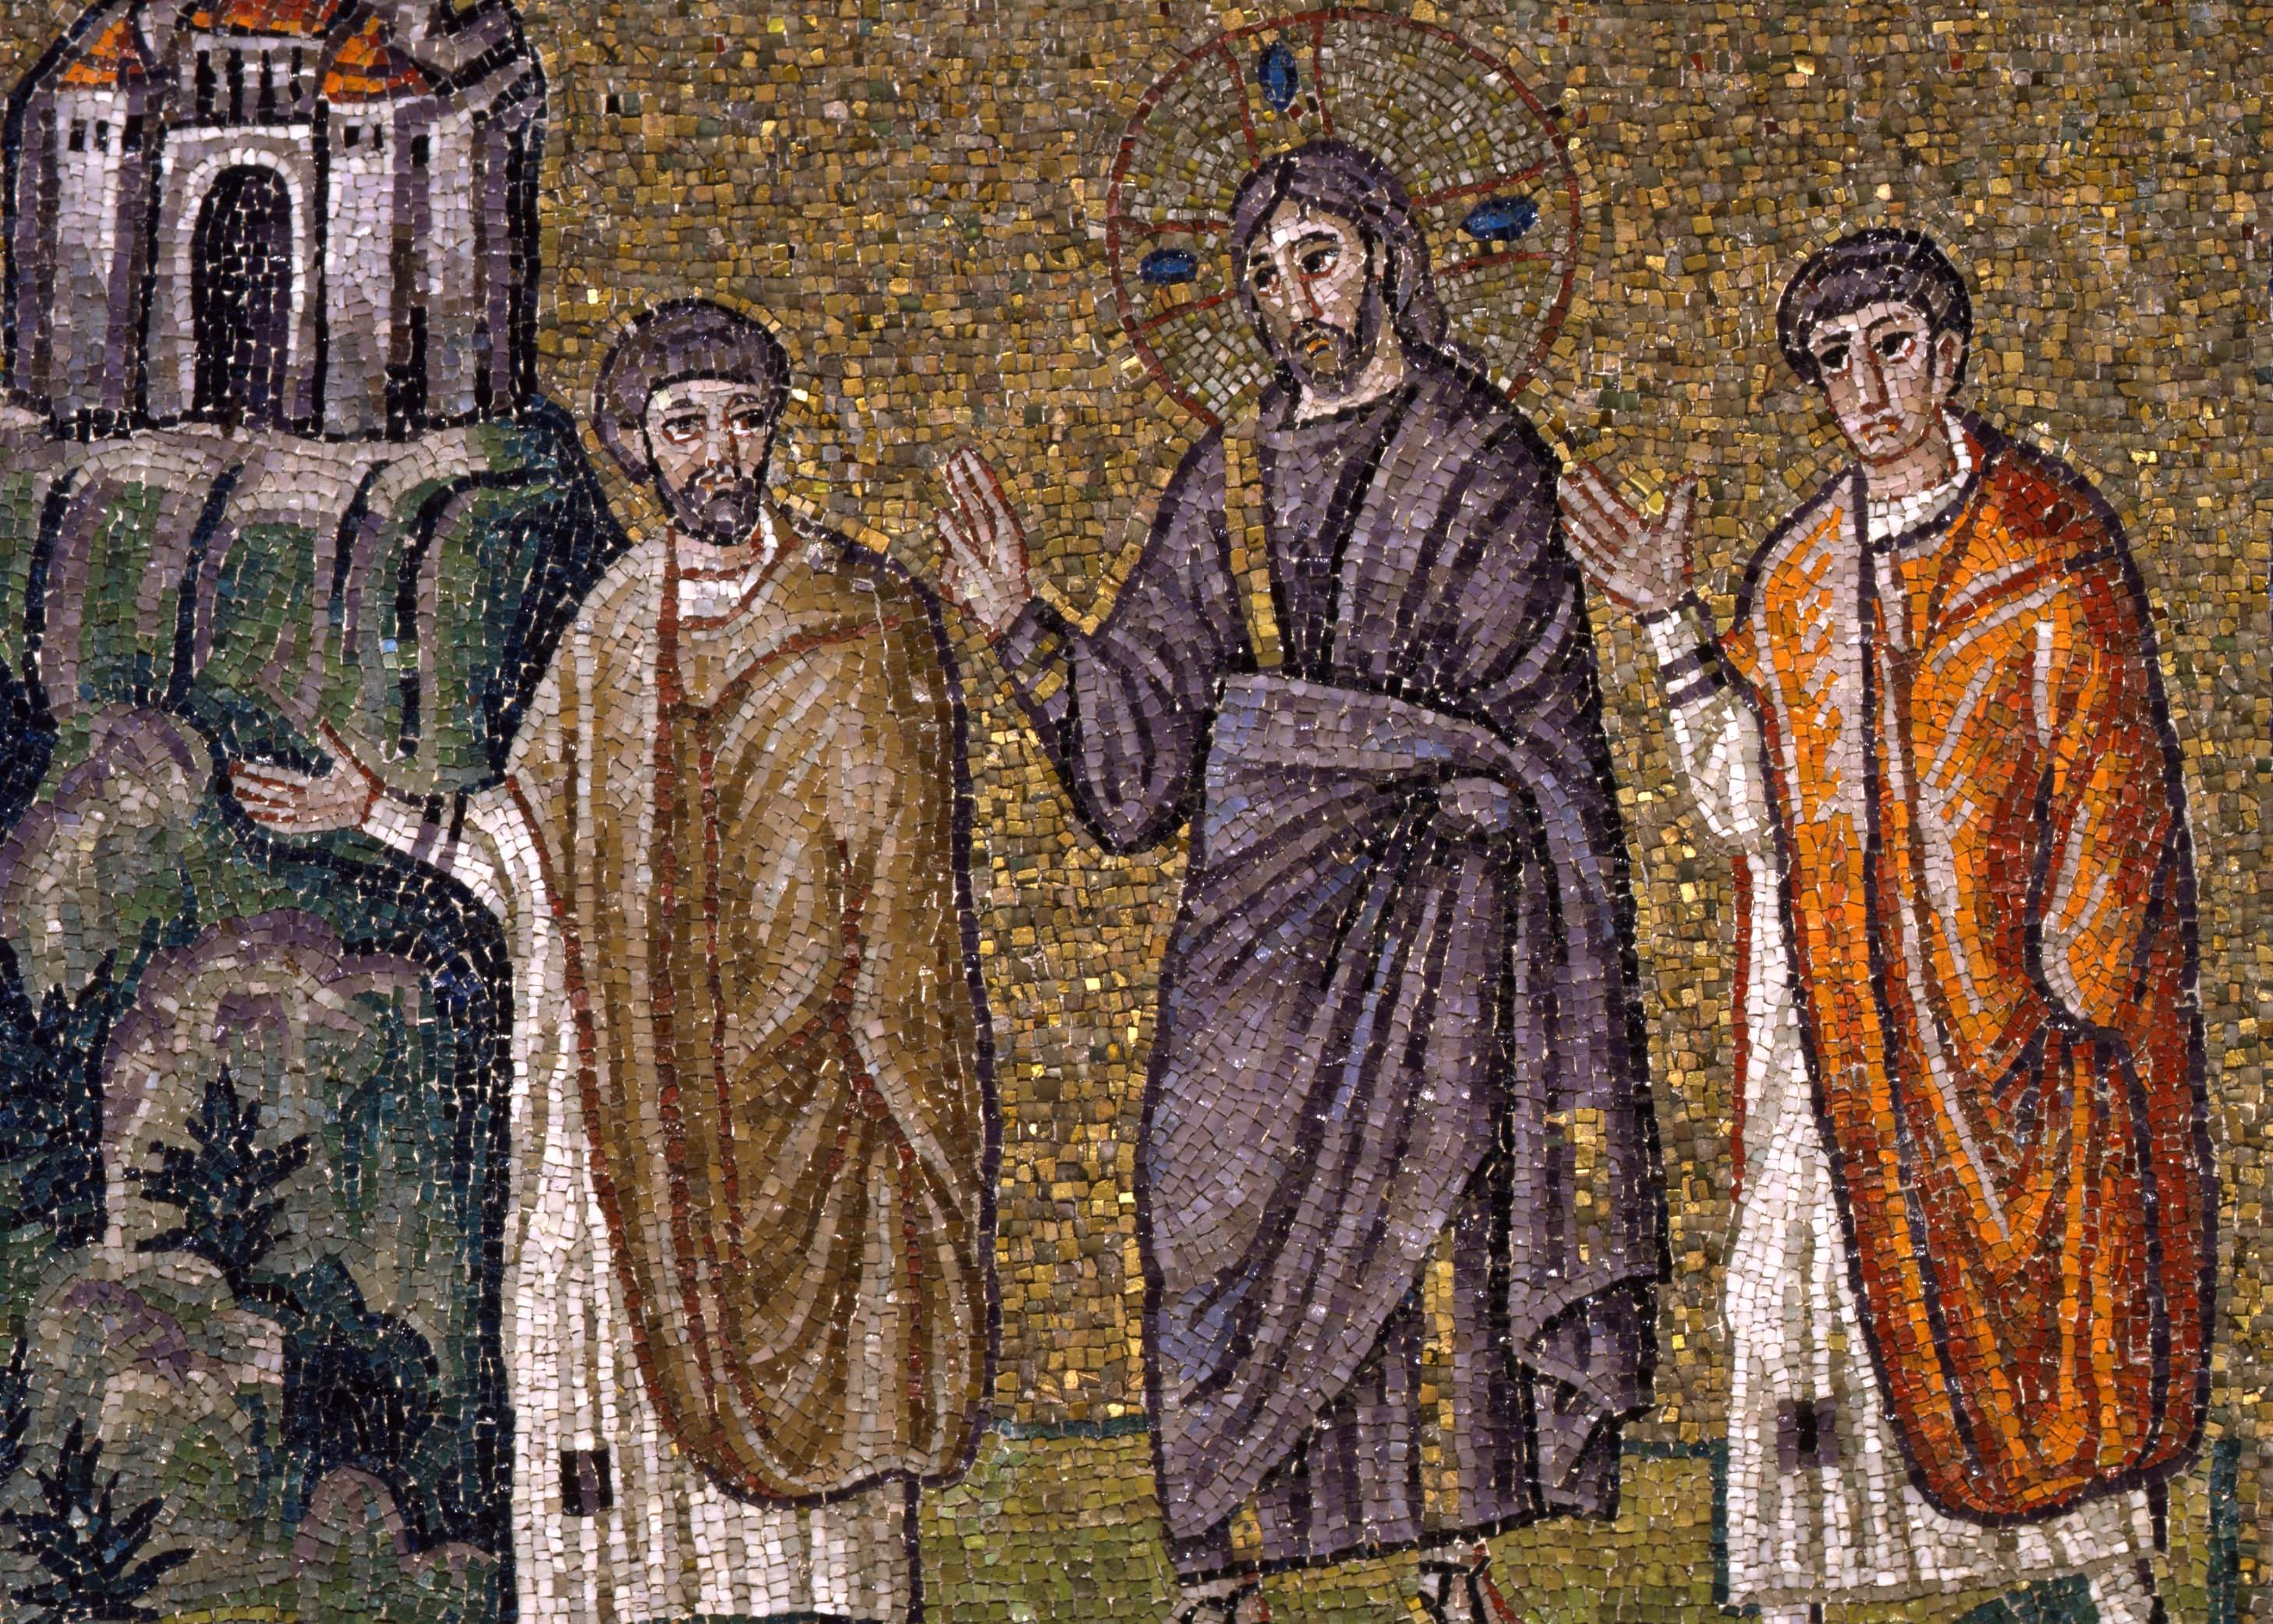
\includegraphics[width=8cm]{emmaus.jpg}
%\end{center}

\vfill

\begin{center}
%Ad usum et secundum consuetudines chori \guillemotright{}Conventus Choralis\guillemotleft.

%Editio Sancti Wolfgangi \annusEditionis
\end{center}

\pagebreak

\renewcommand{\headrulewidth}{0pt} % no horiz. rule at the header
\fancyhf{}
\pagestyle{fancy}

\cantusSineNeumas

\ifx\festumveldominica\undefined
\else
\pars{Oratio ante divinum Officium.}

\lettrine{{\color{red}A}}{peri,} Dómine, os meum ad benedicéndum nomen sanctum tuum:
munda quoque cor meum ab ómnibus vanis, pervérsis, et aliénis
cogitatiónibus:
intelléctum illúmina, afféctum inflámma,
ut digne, atténte ac devóte hoc Offícium recitáre váleam,
et exaudíri mérear ante conspéctum Divínæ Maiestátis tuæ.
Per Christum, Dóminum nostrum.
\Rbardot{} Amen.

Dómine, in unióne illíus divínæ intentiónis,
qua ipse in terris laudes Deo persolvísti,
has tibi Horas \rubricatum{(vel \textnormal{hanc tibi Horam})} persólvo.

%\trOratioAnteOfficium

\vfill

\pars{Oratio post divinum Officium.}

\rubrica{
  Orationem sequentem devote post Officium recitantibus
  Leo Papa X. defectus, et culpas in eo persolvendo ex humana
  fragilitate contractas, indulsit, et dicitur flexis genibus.
}

\lettrine{{\color{red}S}}{acrosánctæ} et indivíduæ Trinitáti,
crucifíxi Dómini nostri Iesu Christi humanitáti,
beatíssimæ et gloriosíssimæ sempérque Vírginis Maríæ
fecúndæ integritáti, 
et ómnium Sanctórum universitáti
sit sempitérna laus, honor, virtus et glória
ab omni creatúra,
nobísque remíssio ómnium peccatórum,
per infiníta sǽcula sæculórum.
\Rbardot{} Amen.

\noindent \Vbardot{} Beáta víscera Maríæ Virginis, quæ portavérunt
ætérni Patris Fílium.\\
\Rbardot{} Et beáta úbera, quæ lactavérunt Christum Dominum.

\rubrica{Et dicitur secreto \textnormal{Pater noster.} et \textnormal{Ave María.}}

%\trOratioPostOfficium

\vfill

\ifx\festum\undefined
\else
\hora{Ad I. Vesperas.} %%%%%%%%%%%%%%%%%%%%%%%%%%%%%%%%%%%%%%%%%%%%%%%%%%%%%
%\sideThumbs{I. Vesperæ}

\vspace{0.5cm}
\grechangedim{interwordspacetext}{0.18 cm plus 0.15 cm minus 0.05 cm}{scalable}%
\ifx\festum\undefined
\cuminitiali{}{temporalia/deusinadiutorium-alter.gtex}
\else
\cuminitiali{}{temporalia/deusinadiutorium-solemnis.gtex}
\fi
\grechangedim{interwordspacetext}{0.22 cm plus 0.15 cm minus 0.05 cm}{scalable}%

\vfill
\pagebreak

\pars{Psalmus 1.} \scriptura{Cf. Lc. 1, 11.13; \textbf{H273}}

\vspace{-0.4cm}

\antiphona{VII a}{temporalia/ant-descenditangelus.gtex}

\scriptura{Psalmus 112.}

\initiumpsalmi{temporalia/ps112-initium-vii-a-auto.gtex}

%\psalmusEtTranslatioT{temporalia/ps112-comb.tex}{10cm}
\input{temporalia/ps112.tex} \Abardot{}

\vspace{-1cm}

\vfill
\pagebreak

\pars{Psalmus 2.} \scriptura{Cf. Lc. 1, 17; \textbf{H275}}

\vspace{-0.4cm}

\antiphona{VII a}{temporalia/ant-ipsepraeibitanteillum.gtex}

\scriptura{Psalmus 116.}

\initiumpsalmi{temporalia/ps116-initium-vii-a-auto.gtex}

%\psalmusEtTranslatioT{temporalia/ps116-comb.tex}{10cm}
\input{temporalia/ps116.tex} \Abardot{}

\vfill
\pagebreak

\pars{Psalmus 3.} \scriptura{Lc. 1, 15.14.63; \textbf{H275}}

\vspace{-0.4cm}

\antiphona{VIII G}{temporalia/ant-joannesest.gtex}

\scriptura{Psalmus 145.}

\initiumpsalmi{temporalia/ps145-initium-viii-G-auto.gtex}

%\psalmusEtTranslatioT{temporalia/ps145-comb.tex}{10cm}
\input{temporalia/ps145.tex} \Abardot{}

\vfill
\pagebreak

\pars{Psalmus 4.} \scriptura{Lc. 1, 36.16; \textbf{H275}}

\vspace{-0.4cm}

\antiphona{I f}{temporalia/ant-exuterosenectutis.gtex}

\scriptura{Psalmus 146.}

\initiumpsalmi{temporalia/ps146-initium-i-f-auto.gtex}

%\psalmusEtTranslatioT{temporalia/ps146-comb.tex}{10cm}
\input{temporalia/ps146.tex} \Abardot{}

\vfill
\pagebreak

\pars{Psalmus 5.} \scriptura{Lc. 1, 15.66; \textbf{H276}}

\vspace{-0.4cm}

\antiphona{VII a}{temporalia/ant-istepuer.gtex}

\scriptura{Psalmus 147.}

\initiumpsalmi{temporalia/ps147-initium-vii-a-auto.gtex}

%\psalmusEtTranslatioT{temporalia/ps147-comb.tex}{10cm}
\input{temporalia/ps147.tex} \Abardot{}

\vfill
\pagebreak

\pars{Capitulum.} \scriptura{Ier. 1, 5}

\grechangedim{interwordspacetext}{0.12 cm plus 0.15 cm minus 0.05 cm}{scalable}%
\cuminitiali{}{temporalia/capitulum-PriusquamTe.gtex}
\grechangedim{interwordspacetext}{0.22 cm plus 0.15 cm minus 0.05 cm}{scalable}

% preklad Jeruz. bible
%\trCapituliI

\vfill

\pars{Responsorium breve.} \scriptura{Cf. Lc. 7, 28}

\cuminitiali{VI}{temporalia/resp-internatos.gtex}

%\trResp

\vfill
\pagebreak

\pars{Hymnus}

\cuminitiali{II}{temporalia/hym-UtQueant.gtex}
\vspace{-3mm}
%\input{hym-UtQueant-bohtext.tex}

\vfill
%\pagebreak

\pars{Versus.} \scriptura{Ps. 91, 13}

% Versus. %%%
\sineinitiali{temporalia/versus-iustus.gtex}

%\noindent \trVersus

\vfill
\pagebreak

\pars{Canticum B. Mariæ V.} \scriptura{Lc. 1, 9.11}

\vspace{-3mm}

{
\grechangedim{interwordspacetext}{0.18 cm plus 0.15 cm minus 0.05 cm}{scalable}%
\antiphona{VIII G}{temporalia/ant-ingressozacharia.gtex}
\grechangedim{interwordspacetext}{0.22 cm plus 0.15 cm minus 0.05 cm}{scalable}%
}

%\trAntIMagnificat

%\vspace{-2mm}

\scriptura{Lc. 1, 46-55}

%\vspace{-2mm}

\cantusSineNeumas
\initiumpsalmi{temporalia/magnificat-initium-viiisoll-G.gtex}

%\psalmusEtTranslatioT{temporalia/magnificat-I-comb.tex}{10.2cm}
\input{temporalia/magnificat-I.tex} \Abardot{}

%\vspace{-1cm}

\vfill
\pagebreak

%\sideThumbs{{\scriptsize{}Fine horarum}}

\anteOrationem

\pagebreak

% Oratio. %%%
\cuminitiali{}{temporalia/oratio.gtex}

\vspace{-1mm}
%\trOrationisI

\vfill

\rubrica{Hebdomadarius dicit iterum Dominus vobiscum, vel cantor dicit:}

\vspace{2mm}

\sineinitiali{temporalia/domineexaudi.gtex}

\rubrica{Postea cantatur a cantore:}

\vspace{2mm}

\ifx\festum\undefined
\cuminitiali{II}{temporalia/benedicamus-semiduplex-vesp.gtex}
\else
\cuminitiali{II}{temporalia/benedicamus-solemnism-1vesp.gtex}
\fi

\vspace{1mm}

\vfill
\pagebreak
\fi

\iffalse
\hora{Ad Matutinum.} %%%%%%%%%%%%%%%%%%%%%%%%%%%%%%%%%%%%%%%%%%%%%%%%%%%%%
%\sideThumbs{Matutinum}

\vspace{2mm}

\cuminitiali{}{temporalia/dominelabiamea.gtex}

\vspace{2mm}

\pars{Invitatorium.} \scriptura{Cantor; \textbf{LU\textsubscript{918}}}

\vspace{-6mm}

\antiphona{IV}{temporalia/inv-christumregemadoremus.gtex}

\vfill
\pagebreak

\pars{Hymnus.}

\vspace{-5mm}

\scriptura{Thomas de Aquino; \textbf{LU\textsubscript{920}}}

\antiphona{IV}{temporalia/hym-SacrisSolemniis.gtex}
%{
%\vspace{-5mm}
%\setlength{\columnsep}{0pt} % prostor mezi sloupci
%\input{hym-SacrisSolemniis-bohtext.tex}
%\setlength{\columnsep}{30pt} % prostor mezi sloupci
%}

\vfill
\pagebreak

\subhora{In I. Nocturno}

\pars{Psalmus 1.} \scriptura{Ps. 1, 3; \textbf{LU\textsubscript{922}}}

\vspace{-2mm}

\antiphona{I D*}{temporalia/ant-fructumsalutiferum.gtex}

%\vspace{-5mm}

\scriptura{Ps. 1}

%\vspace{-2mm}

\initiumpsalmi{temporalia/ps1-initium-i-D_-auto.gtex}

%\psalmusEtTranslatioT{temporalia/ps1-comb.tex}{10cm}
\input{temporalia/ps1.tex} \Abardot{}

\vfill
\pagebreak

\pars{Psalmus 2.} \scriptura{Ps. 4, 8.9; \textbf{LU\textsubscript{923}}}

\vspace{-2mm}

\antiphona{II D}{temporalia/ant-afructufrumenti.gtex}

%\vspace{-5mm}

\scriptura{Ps. 4}

\initiumpsalmi{temporalia/ps4-initium-ii-D-auto.gtex}

%\psalmusEtTranslatioT{temporalia/ps4iiD-comb.tex}{10cm}
\input{temporalia/ps4iiD.tex} \Abardot{}

\vfill
\pagebreak

\pars{Psalmus 3.} \scriptura{Ps. 15, 4; \textbf{LU\textsubscript{924}}}

\vspace{-4mm}

\antiphona{III a\textsuperscript{3}}{temporalia/ant-communionecalicis.gtex}

%\vspace{-2mm}

\scriptura{Ps. 15}

\vspace{-2mm}

\initiumpsalmi{temporalia/ps15-initium-iii-a3-auto.gtex}

%\psalmusEtTranslatioT{temporalia/ps15-comb.tex}{10cm}
\input{temporalia/ps15.tex} \Abardot{}

\vfill
\pagebreak

\pars{Versus.} \scriptura{Sap. 16, 20; Ps. 77, 25}

% Versus. %%%
\sineinitiali{temporalia/versus-panemdecaelohomo-communis.gtex}

\vspace{5mm}

\sineinitiali{temporalia/oratiodominica-mat.gtex}

\vspace{5mm}

\pars{Absolutio.}

\cuminitiali{}{temporalia/absolutio-exaudi.gtex}

\vfill
\pagebreak

\cuminitiali{}{temporalia/benedictio-solemn-benedictione.gtex}

\vspace{7mm}

\lectioi

\noindent \Vbardot{} Tu autem, Dómine, miserére nobis.
\noindent \Rbardot{} Deo grátias.

\vfill
\pagebreak

\pars{Responsorium 1.} \scriptura{\Rbardot{} Ex. 12, 5.6.8 \Vbardot{} 1 Cor. 5, 7.8; \textbf{LU\textsubscript{926}}}

\vspace{-2mm}

\responsorium{I}{temporalia/resp-immolabithaedum.gtex}{}

\vfill
\pagebreak

\cuminitiali{}{temporalia/benedictio-solemn-unigenitus.gtex}

\vspace{7mm}

\lectioii

\noindent \Vbardot{} Tu autem, Dómine, miserére nobis.
\noindent \Rbardot{} Deo grátias.

\vfill
\pagebreak

\pars{Responsorium 2.} \scriptura{\Rbardot{} Ex. 16, 12.15 \Vbardot{} Io. 6, 21; \textbf{LU\textsubscript{927}}}

\vspace{-2mm}

\responsorium{II}{temporalia/resp-comedetiscarnes.gtex}{}

\vfill
\pagebreak

\cuminitiali{}{temporalia/benedictio-solemn-spiritus.gtex}

\vspace{7mm}

\lectioiii

\noindent \Vbardot{} Tu autem, Dómine, miserére nobis.
\noindent \Rbardot{} Deo grátias.

\vfill
\pagebreak

\pars{Responsorium 3.} \scriptura{\Rbardot{} 3 Reg. 19, 6.8 \Vbardot{} Io. 6, 52; \textbf{LU\textsubscript{927}}}

\vspace{-2mm}

\responsorium{III}{temporalia/resp-respexitelias.gtex}{}

\vfill
\pagebreak

\subhora{In II. Nocturno}

\pars{Psalmus 4.} \scriptura{Ps. 19, 4; \textbf{LU\textsubscript{928}}}

\vspace{-2mm}

\antiphona{IV E}{temporalia/ant-memorsit-FKP.gtex}

\vspace{-2mm}

\scriptura{Ps. 19}

\initiumpsalmi{temporalia/ps19-initium-iv-E-auto.gtex}

%\psalmusEtTranslatioT{temporalia/ps19-comb.tex}{10cm}
\input{temporalia/ps19.tex} \Abardot{}

\vfill
\pagebreak

\pars{Psalmus 5.} \scriptura{Ps. 22, 5; \textbf{LU\textsubscript{928}}}

\vspace{-2mm}

\antiphona{V a}{temporalia/ant-paraturnobis-FKP.gtex}

%\vspace{-3mm}

\scriptura{Ps. 22}

%\vspace{-2mm}

\initiumpsalmi{temporalia/ps22-initium-v-a.gtex}

%\vspace{-1.5mm}

%\psalmusEtTranslatioT{temporalia/ps22-comb.tex}{10cm}
\input{temporalia/ps22.tex} \Abardot{}

\vspace{-1cm}

\vfill
\pagebreak

\pars{Psalmus 6.} \scriptura{Ps. 41, 5; \textbf{LU\textsubscript{930}}}

\vspace{-2mm}

\antiphona{VI F}{temporalia/ant-invoceexsultationis-FKP.gtex}

%\vspace{-5mm}

\scriptura{Ps. 41}

\initiumpsalmi{temporalia/ps41-initium-vi-F-auto.gtex}

%\psalmusEtTranslatioT{temporalia/ps41-comb.tex}{10cm}
\input{temporalia/ps41.tex}

\vfill

\antiphona{}{temporalia/ant-invoceexsultationis-FKP.gtex}

\vfill
\pagebreak

\pars{Versus.} \scriptura{Ps. 80, 17}

% Versus. %%%
\sineinitiali{temporalia/versus-cibavit.gtex}

\vspace{5mm}

\sineinitiali{temporalia/oratiodominica-mat.gtex}

\vspace{5mm}

\pars{Absolutio.}

\cuminitiali{}{temporalia/absolutio-ipsius.gtex}

\vfill
\pagebreak

\cuminitiali{}{temporalia/benedictio-solemn-deus.gtex}

\vspace{7mm}

\lectioiv

\noindent \Vbardot{} Tu autem, Dómine, miserére nobis.
\noindent \Rbardot{} Deo grátias.

\vfill
\pagebreak

\pars{Responsorium 4.} \scriptura{\Rbardot{} Mt. 26, 26 \Vbardot{} Io. 31, 31; \textbf{LU\textsubscript{931}}}

\vspace{-2mm}

\responsorium{V}{temporalia/resp-coenantibus.gtex}{}

\vfill
\pagebreak

\cuminitiali{}{temporalia/benedictio-solemn-christus.gtex}

\vspace{7mm}

\lectiov

\noindent \Vbardot{} Tu autem, Dómine, miserére nobis.
\noindent \Rbardot{} Deo grátias.

\vfill
\pagebreak

\pars{Responsorium 5.} \scriptura{\Rbardot{} 1 Cor. 11, 25 \Vbardot{} Thren. 3, 20; \textbf{LU\textsubscript{932}}}

\vspace{-2mm}

\responsorium{VI}{temporalia/resp-accepitiesus.gtex}{}

\vfill
\pagebreak

\cuminitiali{}{temporalia/benedictio-solemn-ignem.gtex}

\vspace{7mm}

\lectiovi

\noindent \Vbardot{} Tu autem, Dómine, miserére nobis.
\noindent \Rbardot{} Deo grátias.

\vfill
\pagebreak

\pars{Responsorium 6.} \scriptura{\Rbardot{} Io. 6, 48 \Vbardot{} ibid. 6, 51.52; \textbf{LU\textsubscript{934}}}

\vspace{-2mm}

\responsorium{VII}{temporalia/resp-egosumpanisvitae.gtex}{}

\vfill
\pagebreak

\subhora{In III. Nocturno}

\pars{Psalmus 7.} \scriptura{Ps. 42, 4; \textbf{LU\textsubscript{934}}}

\vspace{-5mm}

\antiphona{VII a}{temporalia/ant-introibo-FKP.gtex}

\vspace{-4mm}

\scriptura{Ps. 42}

%\vspace{-2mm}

\initiumpsalmi{temporalia/ps42-initium-vii-a-auto.gtex}

%\psalmusEtTranslatioT{temporalia/ps42-comb.tex}{10cm}
\input{temporalia/ps42.tex} \Abardot{}

\vfill
\pagebreak

\pars{Psalmus 8.} \scriptura{Ps. 80, 17; \textbf{LU\textsubscript{935}}}

\vspace{-5mm}

\antiphona{VIII G}{temporalia/ant-cibavitnos-FKP.gtex}

\vspace{-3mm}

\scriptura{Ps. 80}

\vspace{-2mm}

\initiumpsalmi{temporalia/ps80-initium-viii-G-auto.gtex}

\vspace{-1mm}

%\psalmusEtTranslatioT{temporalia/ps80-comb.tex}{10cm}
\input{temporalia/ps80.tex} \Abardot{}

\vfill
\pagebreak

\pars{Psalmus 9.} \scriptura{Ps. 83, 3; \textbf{LU\textsubscript{936}}}

\vspace{-2mm}

\antiphona{VI F}{temporalia/ant-exaltari-FKP.gtex}

\vspace{-2mm}

\scriptura{Ps. 83}

\initiumpsalmi{temporalia/ps83-initium-vi-F-auto.gtex}

%\psalmusEtTranslatioT{temporalia/ps83-comb.tex}{10cm}
\input{temporalia/ps83.tex} \Abardot{}

\vfill
\pagebreak

\pars{Versus.} \scriptura{Ps. 103, 14-15}

% Versus. %%%
\sineinitiali{temporalia/versus-educas.gtex}

\vspace{5mm}

\sineinitiali{temporalia/oratiodominica-mat.gtex}

\vspace{5mm}

\pars{Absolutio.}

\cuminitiali{}{temporalia/absolutio-avinculis.gtex}

\vfill
\pagebreak

\cuminitiali{}{temporalia/benedictio-solemn-evangelica.gtex}

\vspace{7mm}

\lectiovii

\noindent \Vbardot{} Tu autem, Dómine, miserére nobis.
\noindent \Rbardot{} Deo grátias.

\vfill
\pagebreak

\pars{Responsorium 7.} \scriptura{\Rbardot{} Io. 6, 57 \Vbardot{} Dt. 4, 7; \textbf{LU\textsubscript{938}}}

\vspace{-2mm}

\responsorium{VII}{temporalia/resp-quimanducat.gtex}{}

\vfill
\pagebreak

\cuminitiali{}{temporalia/benedictio-solemn-divinum.gtex}

\vspace{7mm}

\lectioviii

\noindent \Vbardot{} Tu autem, Dómine, miserére nobis.
\noindent \Rbardot{} Deo grátias.

\vfill
\pagebreak

\ifx\dominica\undefined
\pars{Responsorium 8.} \scriptura{\Rbardot{} Io. 6, 58 \Vbardot{} Eccli. 15, 3; \textbf{LU\textsubscript{938}}}

\vspace{-2mm}

\responsorium{VIII}{temporalia/resp-misitmevivenspater.gtex}{}
\else
\pars{Responsorium 8.} \scriptura{\Rbardot{} Lc. 14, 16-17 \Vbardot{} Prv. 9, 5}

\vspace{-2mm}

\responsorium{VI}{temporalia/resp-homoquidamfecit.gtex}{}
\fi

\vfill
\pagebreak

\cuminitiali{}{temporalia/benedictio-solemn-adsocietatem.gtex}

\vspace{7mm}

\lectioix

\noindent \Vbardot{} Tu autem, Dómine, miserére nobis.
\noindent \Rbardot{} Deo grátias.

\vfill
\pagebreak

% Te Deum

%\pars{Hymnus Ambrosianus}

\vspace{-5mm}

\ifx\solemnis\undefined
\ifx\aequus\undefined
{
\pars{Hymnus Ambrosianus} \scriptura{Alio modo, iuxta morem Romanum}

\vspace{-2mm}

\grechangedim{interwordspacetext}{0.26 cm plus 0.15 cm minus 0.05 cm}{scalable}%
\cuminitiali{III}{temporalia/tedeum-romanum-gn.gtex}
\grechangedim{interwordspacetext}{0.22 cm plus 0.15 cm minus 0.05 cm}{scalable}%
}
\else
{
\pars{Hymnus Ambrosianus} \scriptura{Tonus Simplex}

\vspace{-2mm}

\grechangedim{interwordspacetext}{0.30 cm plus 0.15 cm minus 0.05 cm}{scalable}%
\cuminitiali{III}{temporalia/tedeum-simplex-gn.gtex}
\grechangedim{interwordspacetext}{0.22 cm plus 0.15 cm minus 0.05 cm}{scalable}%
}
\fi
\else
{
\pars{Hymnus Ambrosianus} \scriptura{Tonus Solemnis}

\vspace{-2mm}

\grechangedim{interwordspacetext}{0.26 cm plus 0.15 cm minus 0.05 cm}{scalable}%
\cuminitiali{III}{temporalia/tedeum-solemnis-gn.gtex}
\grechangedim{interwordspacetext}{0.22 cm plus 0.15 cm minus 0.05 cm}{scalable}%
}
\fi

\vfill
\pagebreak

\rubrica{Reliqua omittuntur, nisi Laudes separandæ sint.}

\sineinitiali{temporalia/domineexaudi.gtex}

\vfill

\pars{Oratio.}

\cuminitiali{}{temporalia/oratio2.gtex}

\vfill

\noindent \Vbardot{} Dómine, exáudi oratiónem meam.
\Rbardot{} Et clamor meus ad te véniat.

\vfill

% Nocturnale Romanum 2002, p. LXXVI Benedicamus Domino seems to match
% the one from Solemn Laudes.
\cuminitiali{V}{temporalia/benedicamus-solemnis-laud.gtex}

\vfill

\noindent \Vbardot{} Fidélium ánimæ per misericórdiam Dei requiéscant in pace.
\Rbardot{} Amen.

\vfill
\pagebreak
\fi

\hora{Ad Laudes.} %%%%%%%%%%%%%%%%%%%%%%%%%%%%%%%%%%%%%%%%%%%%%%%%%%%%%
%\sideThumbs{Laudes}

\cantusSineNeumas

\vspace{0.5cm}
\grechangedim{interwordspacetext}{0.18 cm plus 0.15 cm minus 0.05 cm}{scalable}%
\ifx\festumveldominica\undefined
\cuminitiali{}{temporalia/deusinadiutorium-communis.gtex}
\else
\cuminitiali{}{temporalia/deusinadiutorium-alter.gtex}
\fi
\grechangedim{interwordspacetext}{0.22 cm plus 0.15 cm minus 0.05 cm}{scalable}%

\vfill
%\pagebreak

\pars{Psalmus 1.} \scriptura{Lc. 1, 13; \textbf{H277}}

\vspace{-0.4cm}

\antiphona{III a}{temporalia/ant-elisabethzachariae.gtex}

\scriptura{Psalmus 92.}

\initiumpsalmi{temporalia/ps92-initium-iii-a-auto.gtex}

%\psalmusEtTranslatioT{temporalia/ps92-comb.tex}{10cm}
\input{temporalia/ps92.tex} \Abardot{}

\vfill
\pagebreak

\pars{Psalmus 2.} \scriptura{Lc. 1, 62.63; \textbf{H277}}

\vspace{-0.4cm}

\antiphona{IV E*}{temporalia/ant-innuebantpatriejus.gtex}

\scriptura{Psalmus 99.}

\initiumpsalmi{temporalia/ps99-initium-iv-E_-auto.gtex}

%\psalmusEtTranslatioT{temporalia/ps99-comb.tex}{10cm}
\input{temporalia/ps99.tex} \Abardot{}

\vfill
\pagebreak

\pars{Psalmus 3.} \scriptura{Lc. 1, 13.14; \textbf{H277}}

\vspace{-0.4cm}

\antiphona{I f}{temporalia/ant-joannesvocabitur.gtex}

\scriptura{Psalmus 62.}

\initiumpsalmi{temporalia/ps62-initium-i-f-auto.gtex}

%\psalmusEtTranslatioT{temporalia/ps62-comb.tex}{10cm}
\input{temporalia/ps62.tex} \Abardot{}

\vfill
\pagebreak

\pars{Psalmus 4.} \scriptura{Lc. 7, 28; \textbf{H277}}

\vspace{-0.4cm}

\antiphona{III b}{temporalia/ant-internatosmulierum.gtex}

\scriptura{Canticum trium puerorum, Dan. 3, 57-88 et 56}

\initiumpsalmi{temporalia/dan3-initium-iii-b-auto.gtex}

%\psalmusEtTranslatioT{temporalia/dan3-comb.tex}{10cm}
\input{temporalia/dan3.tex}

\rubrica{Hic non dicitur Gloria Patri, neque Amen.}

\vfill

\vspace{-6mm}

\antiphona{}{temporalia/ant-internatosmulierum.gtex} % repeat the antiphon - new page

\vfill
\pagebreak

\pars{Psalmus 5.} \scriptura{Lc. 1, 76; \textbf{H277}}

\vspace{-0.4cm}

\antiphona{III b}{temporalia/ant-tupuerpropheta.gtex}

\scriptura{Psalmus 148.}

\initiumpsalmi{temporalia/ps148-initium-iii-b-auto.gtex}

%\psalmusEtTranslatioT{temporalia/ps148-comb.tex}{10cm}
\input{temporalia/ps148.tex}

\rubrica{Hic non dicitur Gloria Patri.}

\vfill
\pagebreak

%
\scriptura{Psalmus 149.}

\initiumpsalmi{temporalia/ps149-initium-iii-b-auto.gtex}

%\psalmusEtTranslatioT{temporalia/ps149-comb.tex}{10cm}
\input{temporalia/ps149.tex}

\rubrica{Hic non dicitur Gloria Patri.}

\vfill
\pagebreak

%
\scriptura{Psalmus 150.}

\initiumpsalmi{temporalia/ps150-initium-iii-b-auto.gtex}

%\psalmusEtTranslatioT{temporalia/ps150-comb.tex}{10cm}
\input{temporalia/ps150.tex}

\vfill

\vspace{-6mm}

\antiphona{}{temporalia/ant-tupuerpropheta.gtex} % repeat the antiphon - new page

\vfill
\pagebreak

\pars{Capitulum.} \scriptura{Is. 49, 1}

\grechangedim{interwordspacetext}{0.12 cm plus 0.15 cm minus 0.05 cm}{scalable}%
\cuminitiali{}{temporalia/capitulum-HaecDicit.gtex}
\grechangedim{interwordspacetext}{0.22 cm plus 0.15 cm minus 0.05 cm}{scalable}

% preklad Jeruz. bible
%\trCapituliI

\vfill

\pars{Responsorium breve.} \scriptura{Cf. Lc. 7, 28}

\ifx\festum\undefined
\cuminitiali{VI}{temporalia/resp-internatos-communis.gtex}
\else
\cuminitiali{VI}{temporalia/resp-internatos.gtex}
\fi

%\trResp

\vfill
\pagebreak

\pars{Hymnus}

\cuminitiali{IV}{temporalia/hym-ONimis.gtex}
\vspace{-3mm}
%\input{hym-ONimis-bohtext.tex}

\vfill
%\pagebreak

\pars{Versus.} \scriptura{Ps. 91, 13}

% Versus. %%%
\sineinitiali{temporalia/versus-iustus.gtex}

%\noindent \trVersus

\vfill
\pagebreak

\pars{Canticum Zachariæ.} \scriptura{Lc. 1, 64.67.68; \textbf{H277}}

\vspace{-4mm}

{
\grechangedim{interwordspacetext}{0.18 cm plus 0.15 cm minus 0.05 cm}{scalable}%
\antiphona{VIII G}{temporalia/ant-apertumestoszachariae.gtex}
\grechangedim{interwordspacetext}{0.22 cm plus 0.15 cm minus 0.05 cm}{scalable}%
}

%\trAntIMagnificat

\vspace{-2mm}

\scriptura{Lc. 1, 68-79}

\vspace{-1mm}

\cantusSineNeumas
\ifx\solemnis\undefined
\initiumpsalmi{temporalia/benedictus-initium-viii-G-auto.gtex}

%\vspace{-1.5mm}

%\psalmusEtTranslatioT{temporalia/benedictus-III-comb.tex}{10.2cm}
\input{temporalia/benedictus-III.tex} \Abardot{}
\else
\initiumpsalmi{temporalia/benedictus-initium-viiisoll-G-auto.gtex}

%\vspace{-1.5mm}

%\psalmusEtTranslatioT{temporalia/benedictus-I-comb.tex}{10.2cm}
\input{temporalia/benedictus-I.tex} \Abardot{}
\fi

\vspace{-1cm}

\vfill
\pagebreak

%\sideThumbs{{\scriptsize{}Fine horarum}}

\anteOrationem

\pagebreak

% Oratio. %%%
\cuminitiali{}{temporalia/oratio2.gtex}

\vspace{-1mm}
%\trOrationisI

\vfill

\rubrica{Hebdomadarius dicit iterum Dominus vobiscum, vel cantor dicit:}

\vspace{2mm}

\sineinitiali{temporalia/domineexaudi.gtex}

\rubrica{Postea cantatur a cantore:}

\vspace{2mm}

\ifx\festum\undefined
\ifx\octava\undefined
\cuminitiali{I}{temporalia/benedicamus-semiduplex-laud.gtex}
\else
\cuminitiali{VIII}{temporalia/benedicamus-duplexmajus-laudes.gtex}
\fi
\else
\cuminitiali{II}{temporalia/benedicamus-solemnism-laud.gtex}
\fi

\vspace{1mm}

\vfill
\pagebreak

\ifx\sabbatoveloctava\undefined
\ifx\festumveldominica\undefined
\hora{Ad Vesperas.} %%%%%%%%%%%%%%%%%%%%%%%%%%%%%%%%%%%%%%%%%%%%%%%%%%%%%
%\sideThumbs{Vesperæ}
\else
\hora{Ad II. Vesperas.} %%%%%%%%%%%%%%%%%%%%%%%%%%%%%%%%%%%%%%%%%%%%%%%%%%%%%
%\sideThumbs{II. Vesperæ}
\fi

\cantusSineNeumas

%\vspace{-2mm}
\grechangedim{interwordspacetext}{0.18 cm plus 0.15 cm minus 0.05 cm}{scalable}%
\ifx\festumveldominica\undefined
\cuminitiali{}{temporalia/deusinadiutorium-communis.gtex}
\else
\ifx\festum\undefined
\cuminitiali{}{temporalia/deusinadiutorium-alter.gtex}
\else
\cuminitiali{}{temporalia/deusinadiutorium-solemnis.gtex}
\fi
\fi
\grechangedim{interwordspacetext}{0.22 cm plus 0.15 cm minus 0.05 cm}{scalable}%

\vfill
%\pagebreak

%\vspace{-2mm}

\pars{Psalmus 1.} \scriptura{Lc. 1, 13; \textbf{H277}}

\vspace{-0.4cm}

\antiphona{III a}{temporalia/ant-elisabethzachariae.gtex}

\scriptura{Psalmus 109.}

\initiumpsalmi{temporalia/ps109-initium-iii-a-auto.gtex}

%\psalmusEtTranslatioT{temporalia/ps109-comb.tex}{10cm}
\input{temporalia/ps109.tex} \Abardot{}

\vfill
\pagebreak

\pars{Psalmus 2.} \scriptura{Lc. 1, 62.63; \textbf{H277}}

\vspace{-0.4cm}

\antiphona{IV E*}{temporalia/ant-innuebantpatriejus.gtex}

\scriptura{Psalmus 110.}

\initiumpsalmi{temporalia/ps110-initium-iv-E_-auto.gtex}

%\psalmusEtTranslatioT{temporalia/ps110-comb.tex}{10cm}
\input{temporalia/ps110.tex} \Abardot{}

\vfill
\pagebreak

\pars{Psalmus 3.} \scriptura{Lc. 1, 13.14; \textbf{H277}}

\vspace{-0.4cm}

\antiphona{I f}{temporalia/ant-joannesvocabitur.gtex}

\scriptura{Psalmus 111.}

\initiumpsalmi{temporalia/ps111-initium-i-f-auto.gtex}

%\psalmusEtTranslatioT{temporalia/ps111-comb.tex}{10cm}
\input{temporalia/ps111.tex} \Abardot{}

\vfill
\pagebreak

\pars{Psalmus 4.} \scriptura{Lc. 7, 28; \textbf{H277}}

\vspace{-0.4cm}

\antiphona{III b}{temporalia/ant-internatosmulierum.gtex}

\scriptura{Psalmus 129.}

\initiumpsalmi{temporalia/ps129-initium-iii-b-auto.gtex}

%\psalmusEtTranslatioT{temporalia/ps129-comb.tex}{10cm}
\input{temporalia/ps129.tex} \Abardot{}

\vfill
\pagebreak

\pars{Psalmus 5.} \scriptura{Lc. 1, 76; \textbf{H277}}

\vspace{-0.4cm}

\antiphona{III b}{temporalia/ant-tupuerpropheta.gtex}

\scriptura{Psalmus 131.}

\initiumpsalmi{temporalia/ps131-initium-iii-b-auto.gtex}

%\psalmusEtTranslatioT{temporalia/ps131-comb.tex}{10cm}
\input{temporalia/ps131.tex}

\vfill

\antiphona{}{temporalia/ant-tupuerpropheta.gtex}

\vfill
\pagebreak

\pars{Capitulum.} \scriptura{Is. 49, 7}

\grechangedim{interwordspacetext}{0.12 cm plus 0.15 cm minus 0.05 cm}{scalable}%
\cuminitiali{}{temporalia/capitulum-RegesVidebunt.gtex}
\grechangedim{interwordspacetext}{0.22 cm plus 0.15 cm minus 0.05 cm}{scalable}

% preklad Jeruz. bible
%\trCapituliI

\vfill

\pars{Responsorium breve.} \scriptura{Cf. Lc. 7, 28}

\cuminitiali{VI}{temporalia/resp-internatos.gtex}

%\trResp

\vfill
\pagebreak

\pars{Hymnus}

\cuminitiali{II}{temporalia/hym-UtQueant.gtex}
\vspace{-3mm}
%\input{hym-UtQueant-bohtext.tex}

\vfill
%\pagebreak

\pars{Versus.} \scriptura{Ps. 91, 13}

% Versus. %%%
\sineinitiali{temporalia/versus-iustus.gtex}

%\noindent \trVersus

\vfill
\pagebreak

\pars{Canticum B. Mariæ V.} \scriptura{Ier. 20, 15; Lc. 7, 28; \textbf{H277}}

\vspace{-6mm}

{
\grechangedim{interwordspacetext}{0.18 cm plus 0.15 cm minus 0.05 cm}{scalable}%
\antiphona{VII d}{temporalia/ant-puerquinatusest.gtex}
\grechangedim{interwordspacetext}{0.22 cm plus 0.15 cm minus 0.05 cm}{scalable}%
}

%\trAntIMagnificat

\vspace{-3mm}

\scriptura{Lc. 1, 46-55}

\vspace{-2.5mm}

\cantusSineNeumas
\ifx\solemnis\undefined
\initiumpsalmi{temporalia/magnificat-initium-vii-a.gtex}

\vspace{-1.5mm}

%\psalmusEtTranslatioT{temporalia/magnificat-V-comb.tex}{10.2cm}
\input{temporalia/magnificat-V.tex} \Abardot{}
\else
\initiumpsalmi{temporalia/magnificat-initium-viisoll-a.gtex}

\vspace{-1.5mm}

%\psalmusEtTranslatioT{temporalia/magnificat-II-comb.tex}{10.2cm}
\input{temporalia/magnificat-II.tex} \Abardot{}
\fi

\vspace{-1cm}

\vfill
\pagebreak

%\sideThumbs{{\scriptsize{}Fine horarum}}

\anteOrationem

\pagebreak

% Oratio. %%%
\cuminitiali{}{temporalia/oratio2.gtex}

\vspace{-1mm}
%\trOrationisI

\vfill

\rubrica{Hebdomadarius dicit iterum Dominus vobiscum, vel cantor dicit:}

\vspace{2mm}

\sineinitiali{temporalia/domineexaudi.gtex}

\rubrica{Postea cantatur a cantore:}

\vspace{2mm}

\ifx\festum\undefined
\cuminitiali{II}{temporalia/benedicamus-semiduplex-vesp.gtex}
\else
\cuminitiali{II}{temporalia/benedicamus-solemnism-2vesp.gtex}
\fi

\vspace{1mm}
\fi

\end{document}

